\documentclass{beamer}

\mode<presentation> {
	% The Beamer class comes with a number of default slide themes
	% which change the colors and layouts of slides. Below this is a list
	% of all the themes, uncomment each in turn to see what they look like.
	
	%\usetheme{default}
	%\usetheme{AnnArbor}
	%\usetheme{Antibes}
	%\usetheme{Bergen}
	%\usetheme{Berkeley}
	%\usetheme{Berlin}
	%\usetheme{Boadilla}
	%\usetheme{CambridgeUS}
	%\usetheme{Copenhagen}
	%\usetheme{Darmstadt}
	%\usetheme{Dresden}
	%\usetheme{Frankfurt}
	%\usetheme{Goettingen}
	%\usetheme{Hannover}
	%\usetheme{Ilmenau}
	%\usetheme{JuanLesPins}
	%\usetheme{Luebeck}
	\usetheme{Madrid}
	%\usetheme{Malmoe}
	%\usetheme{Marburg}
	%\usetheme{Montpellier}
	%\usetheme{PaloAlto}
	%\usetheme{Pittsburgh}
	%\usetheme{Rochester}
	%\usetheme{Singapore}
	%\usetheme{Szeged}
	%\usetheme{Warsaw}
	
	% As well as themes, the Beamer class has a number of color themes
	% for any slide theme. Uncomment each of these in turn to see how it
	% changes the colors of your current slide theme.
	
	%\usecolortheme{albatross}
	\usecolortheme{beaver}
	%\usecolortheme{beetle}
	%\usecolortheme{crane}
	%\usecolortheme{dolphin}
	%\usecolortheme{dove}
	%\usecolortheme{fly}
	%\usecolortheme{lily}
	%\usecolortheme{orchid}
	%\usecolortheme{rose}
	%\usecolortheme{seagull}
	%\usecolortheme{seahorse}
	%\usecolortheme{whale}
	%\usecolortheme{wolverine}
	
	%\setbeamertemplate{footline} % To remove the footer line in all slides uncomment this line
	%\setbeamertemplate{footline}[page number] % To replace the footer line in all slides with a simple slide count uncomment this line
	
	%\setbeamertemplate{navigation symbols}{} % To remove the navigation symbols from the bottom of all slides uncomment this line
}
\usepackage[natbib=true,backend=bibtex,useprefix=true]{biblatex}
\addbibresource{reference.bib}
\setbeamertemplate{caption}[numbered]
\newcommand{\btVFill}{\vskip0pt plus 1filll}
\usepackage{algorithm}
\usepackage{amsmath}
\usepackage{caption}
\usepackage{fec}
\usepackage{xcolor}
%----------------------------------------------------------------------------------------
%	TITLE PAGE
%----------------------------------------------------------------------------------------

\title[Warm Starting Series of MILP's]{Warm Starting Series of Mixed-Integer Linear Programs}

\author{Sean Kelley} % Your name
\date{10 March 2022} % Date, can be changed to a custom date

\begin{document}
	
	\begin{frame}
		\titlepage % Print the title page as the first slide
	\end{frame}

	\begin{frame}{Overview}
		\tableofcontents
	\end{frame}

	\section{Why care about series of MILP's?}
	
	\begin{frame}[t]
		\frametitle{Motivation}
		\small
		\begin{itemize}
			\item Mixed-Integer Programming has created great value in industry.
			\item One important source comes from problems solved by a series of Mixed-Integer Linear Programs (MILPs).
			\begin{itemize}
				\item Electric Grid Production Planning (Stochastic Dual Decomposition)
				\item Vehicle Routing (Branch and Price)
			\end{itemize}
			\item Many MILP instances in such series differ only by objective coefficients or bounds on their constraints.
			\item Solvers can leverage what they discover solving one MILP to more quickly solve a similar MILP (a.k.a. "Warm Start").
			\item Warm starting would enable greater performance and expand the space of tractable problems for those solved as a series of MILPs.
		\end{itemize}
		\vspace{-.25cm}
		\begin{block}{}
			More problems are solved as series of MILP's than meet the eye. Given their economic importance, it is worth understanding how to solve them efficiently.
		\end{block}
		\normalsize
	\end{frame}

	\section{What opportunity is there to more efficiently solve series of MILP's?}

	\begin{frame}[t]
		\frametitle{Simple Example}
		\footnotesize
		% what kind of information can a solver glean from a previous similar solve
		% two MILP's and their trees
		% Plug (2)'s bounds into (1)'s subproblems (get the right)
		% Gives us a branching decision (disjunction), primal solutions and dual bounds
		% Get similar tree by plugging in new objective instead of bounds
		\begin{columns}[T]
			\begin{column}{0.45\textwidth}
				\vspace{-.75cm}
				\begin{align}
					\begin{split}
						\text{max} \{ &x + 4y : -\frac{x}{2} + y \leq 2, \\
						&x + \frac{y}{2} \leq 4, (x, y) \in \Zmbb^2_+ \} 
					\end{split}
					\label{left}
				\end{align}
				\vspace{-.5cm}
				\begin{figure}[h]
					\resizebox{.45\textwidth}{!}{%
						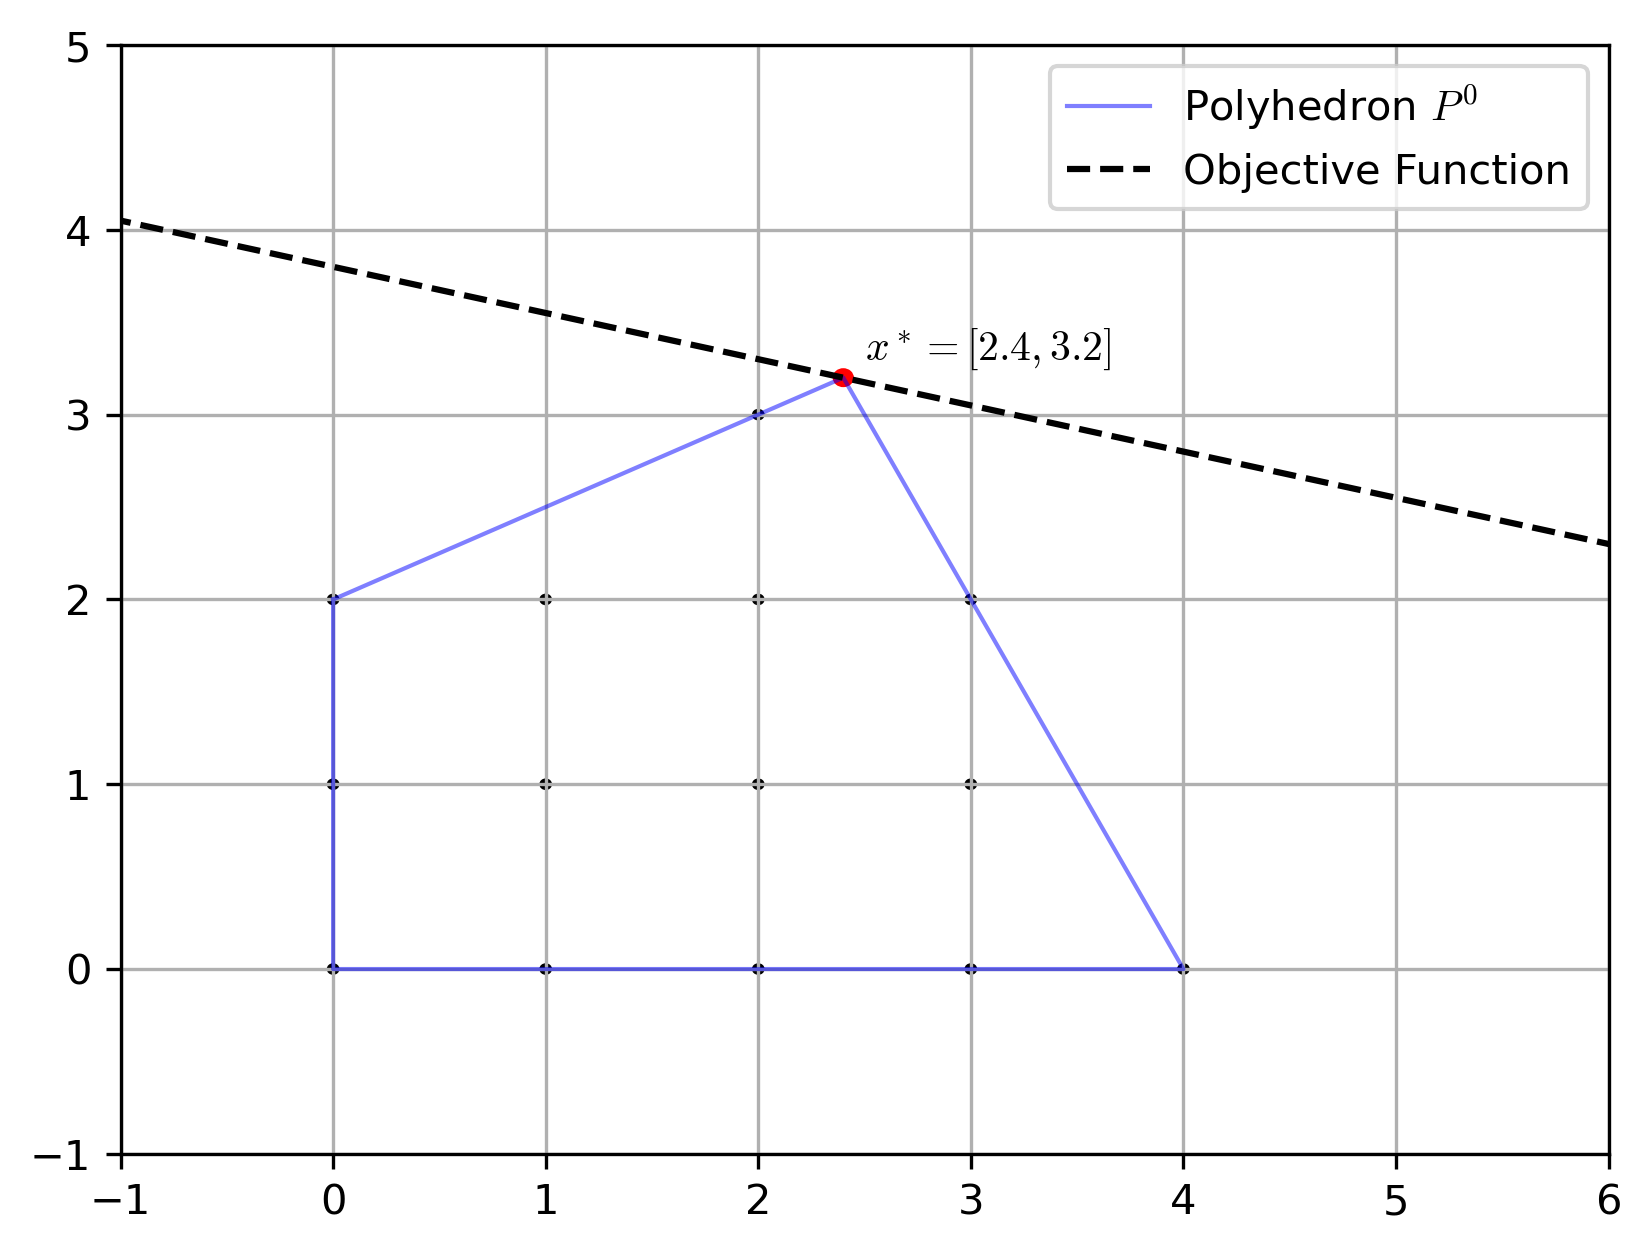
\includegraphics[]{P0.png}
					}
					% \caption{Node 0 LP relaxation}
					\label{p:root}
				\end{figure}
				\centering
				Branch on $ x \leq 2 $ or $ x \geq 3 $
				\begin{figure}[]
					\centering
					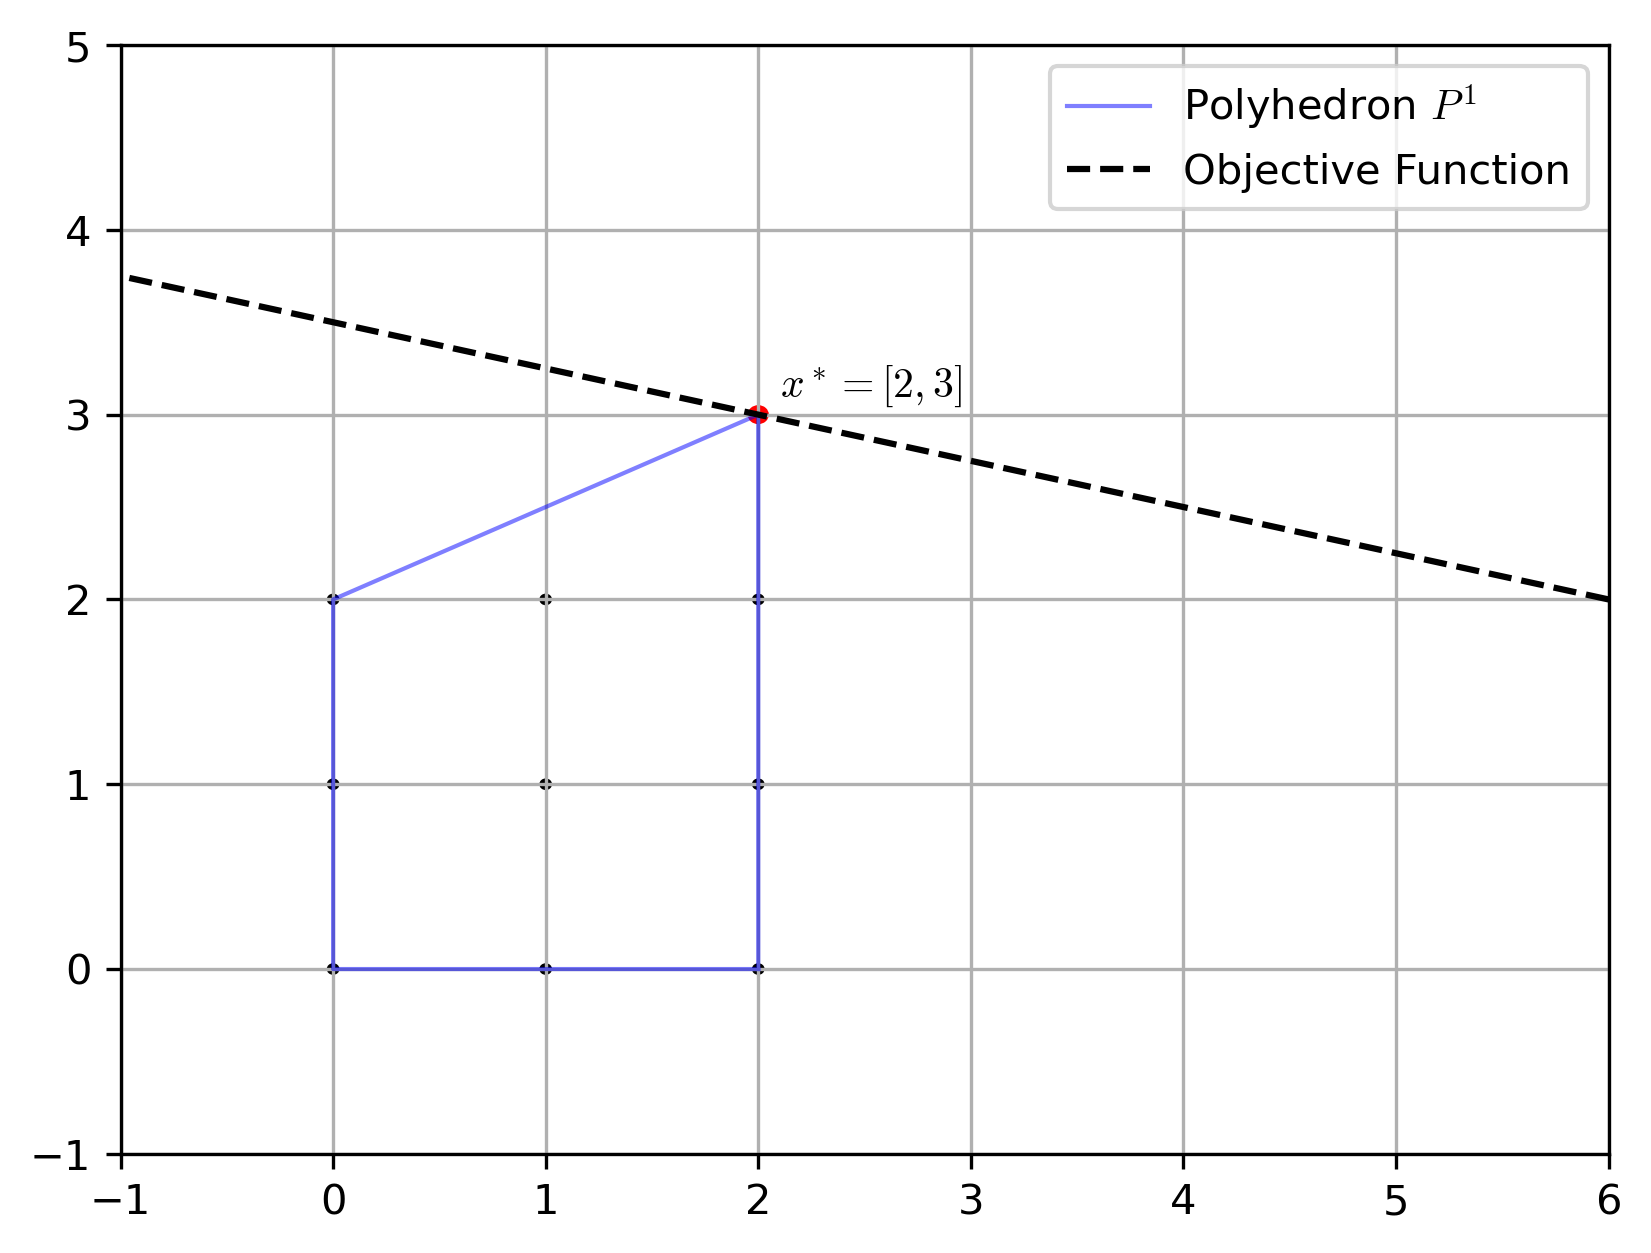
\includegraphics[width=.45\textwidth]{P1.png}
					\hfill
					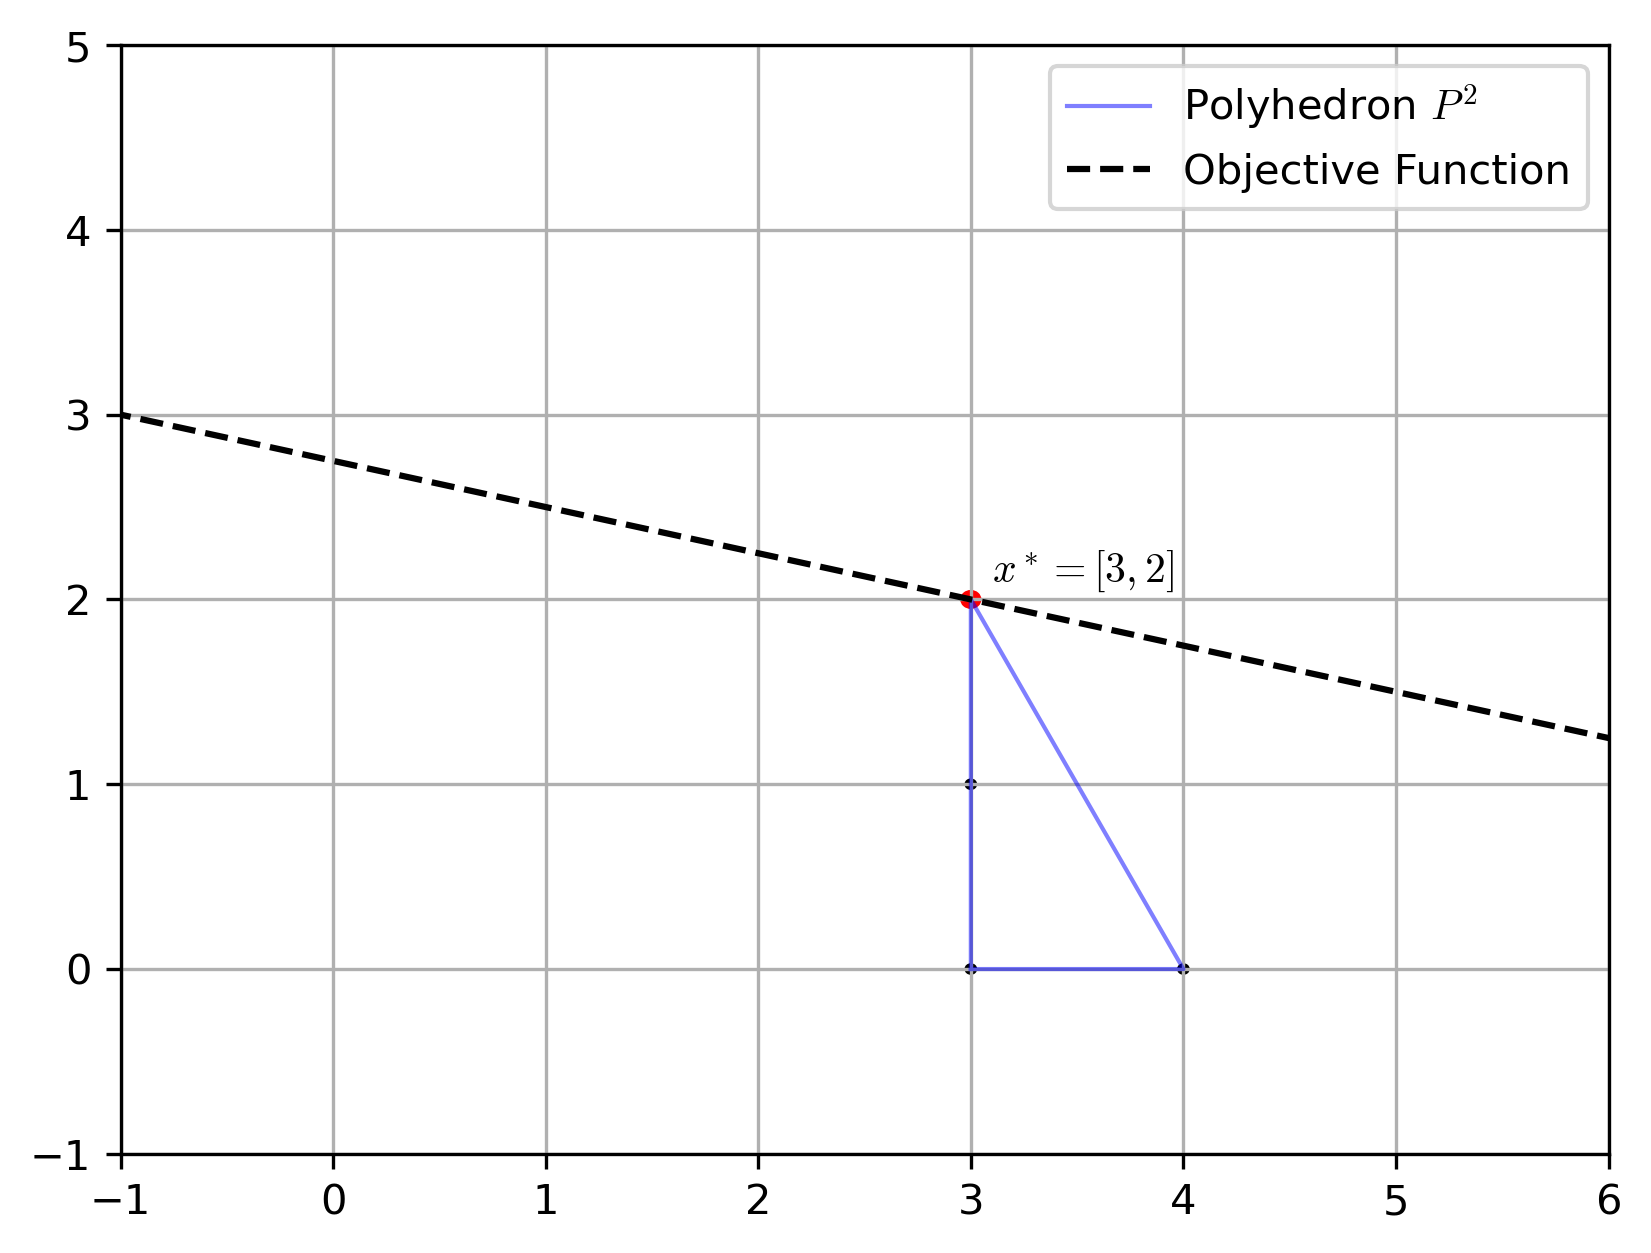
\includegraphics[width=.45\textwidth]{P2.png}
					\captionsetup{font=footnotesize,labelfont=footnotesize}
					\caption{(\ref{left})'s Branch and Bound tree}
					\label{p:before}
				\end{figure}
			\end{column}
			\begin{column}{0.10\textwidth}
				\vspace{2.5cm}
				\centering
				Update bounds $ \implies $
			\end{column}
			\begin{column}{0.45\textwidth}
				\vspace{-.75cm}
				\begin{align}
					\begin{split}
						\text{max} \{ &x + 4y : -\frac{x}{2} + y \leq 3, \\
						&x + \frac{y}{2} \leq 5, (x, y) \in \Zmbb^2_+ \} 
					\end{split}
					\label{right}
				\end{align}
				\vspace{-.5cm}
				\begin{figure}[h]
					\resizebox{.45\textwidth}{!}{%
						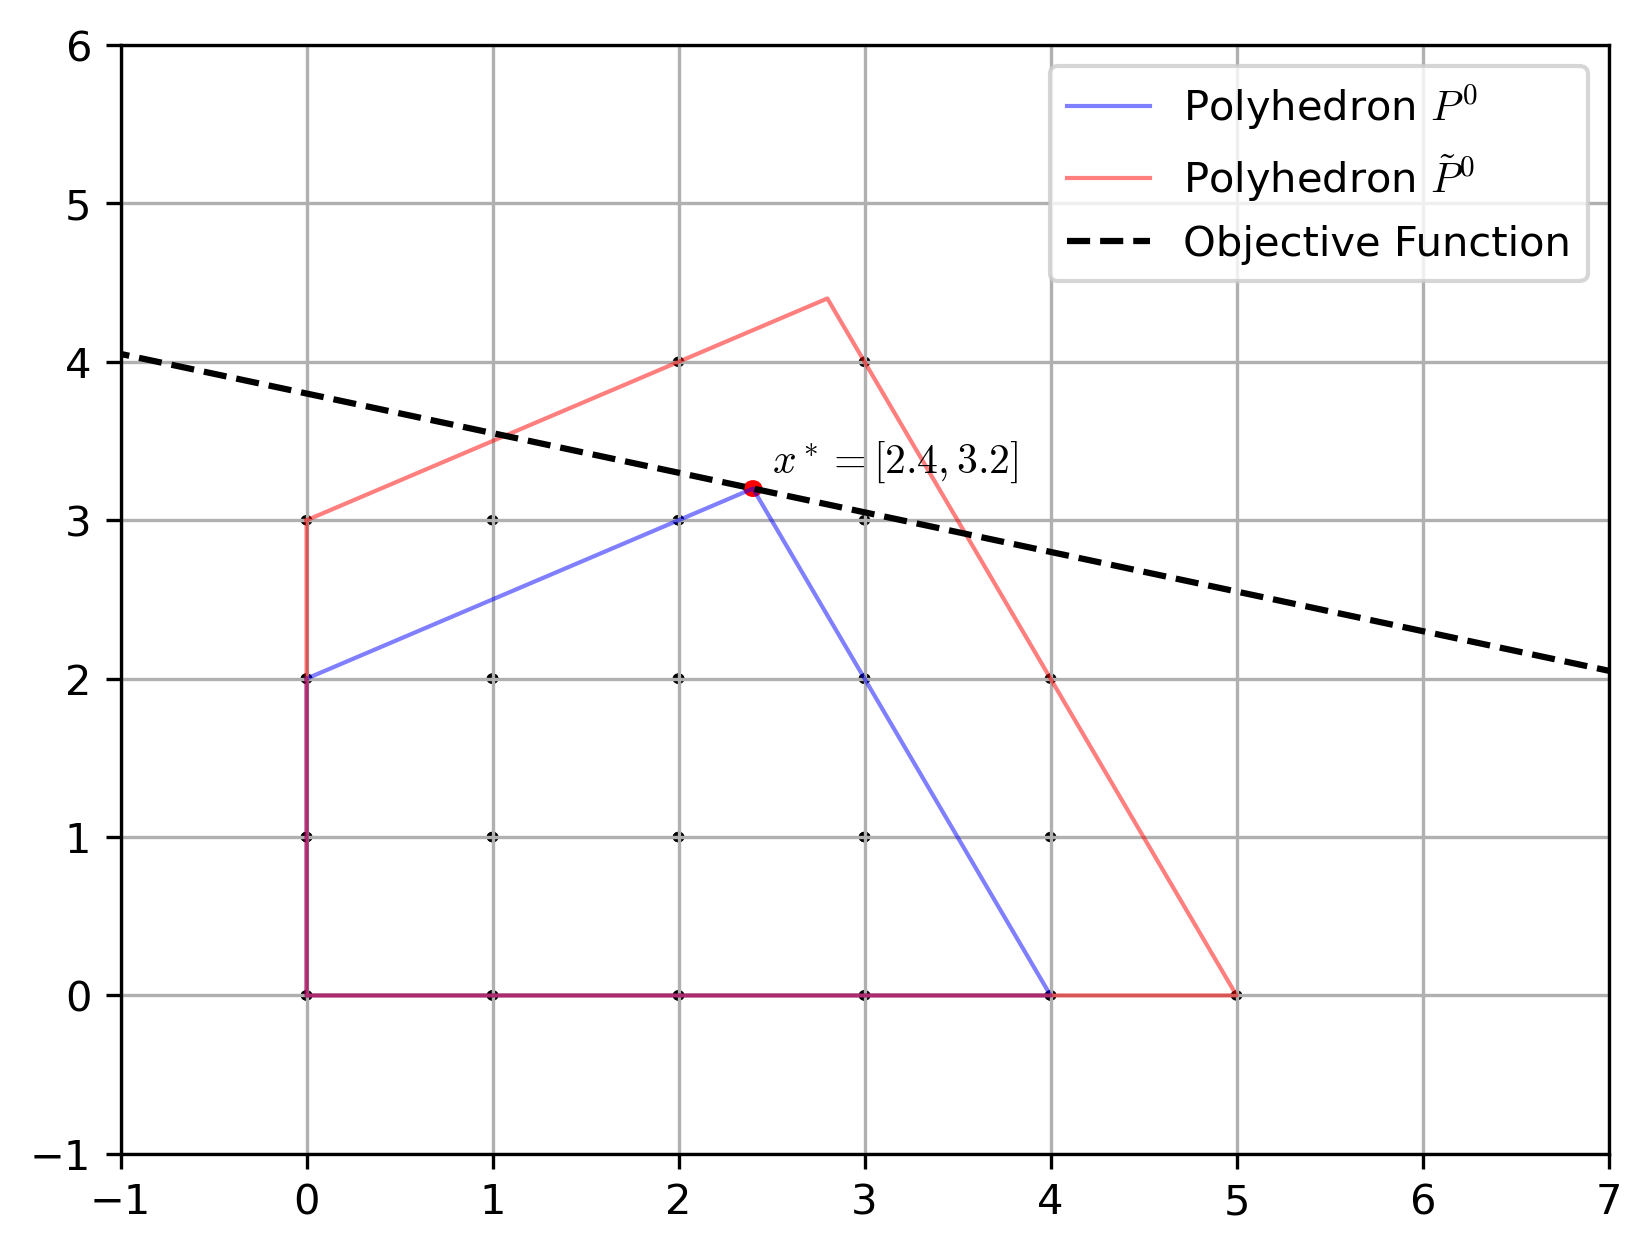
\includegraphics[]{P0_prime.png}
					}
					% \caption{Node 0 LP relaxation}
					\label{p:root_prime}
				\end{figure}
				\centering
				Branch on $ x \leq 2 $ or $ x \geq 3 $
				\begin{figure}[]
					\centering
					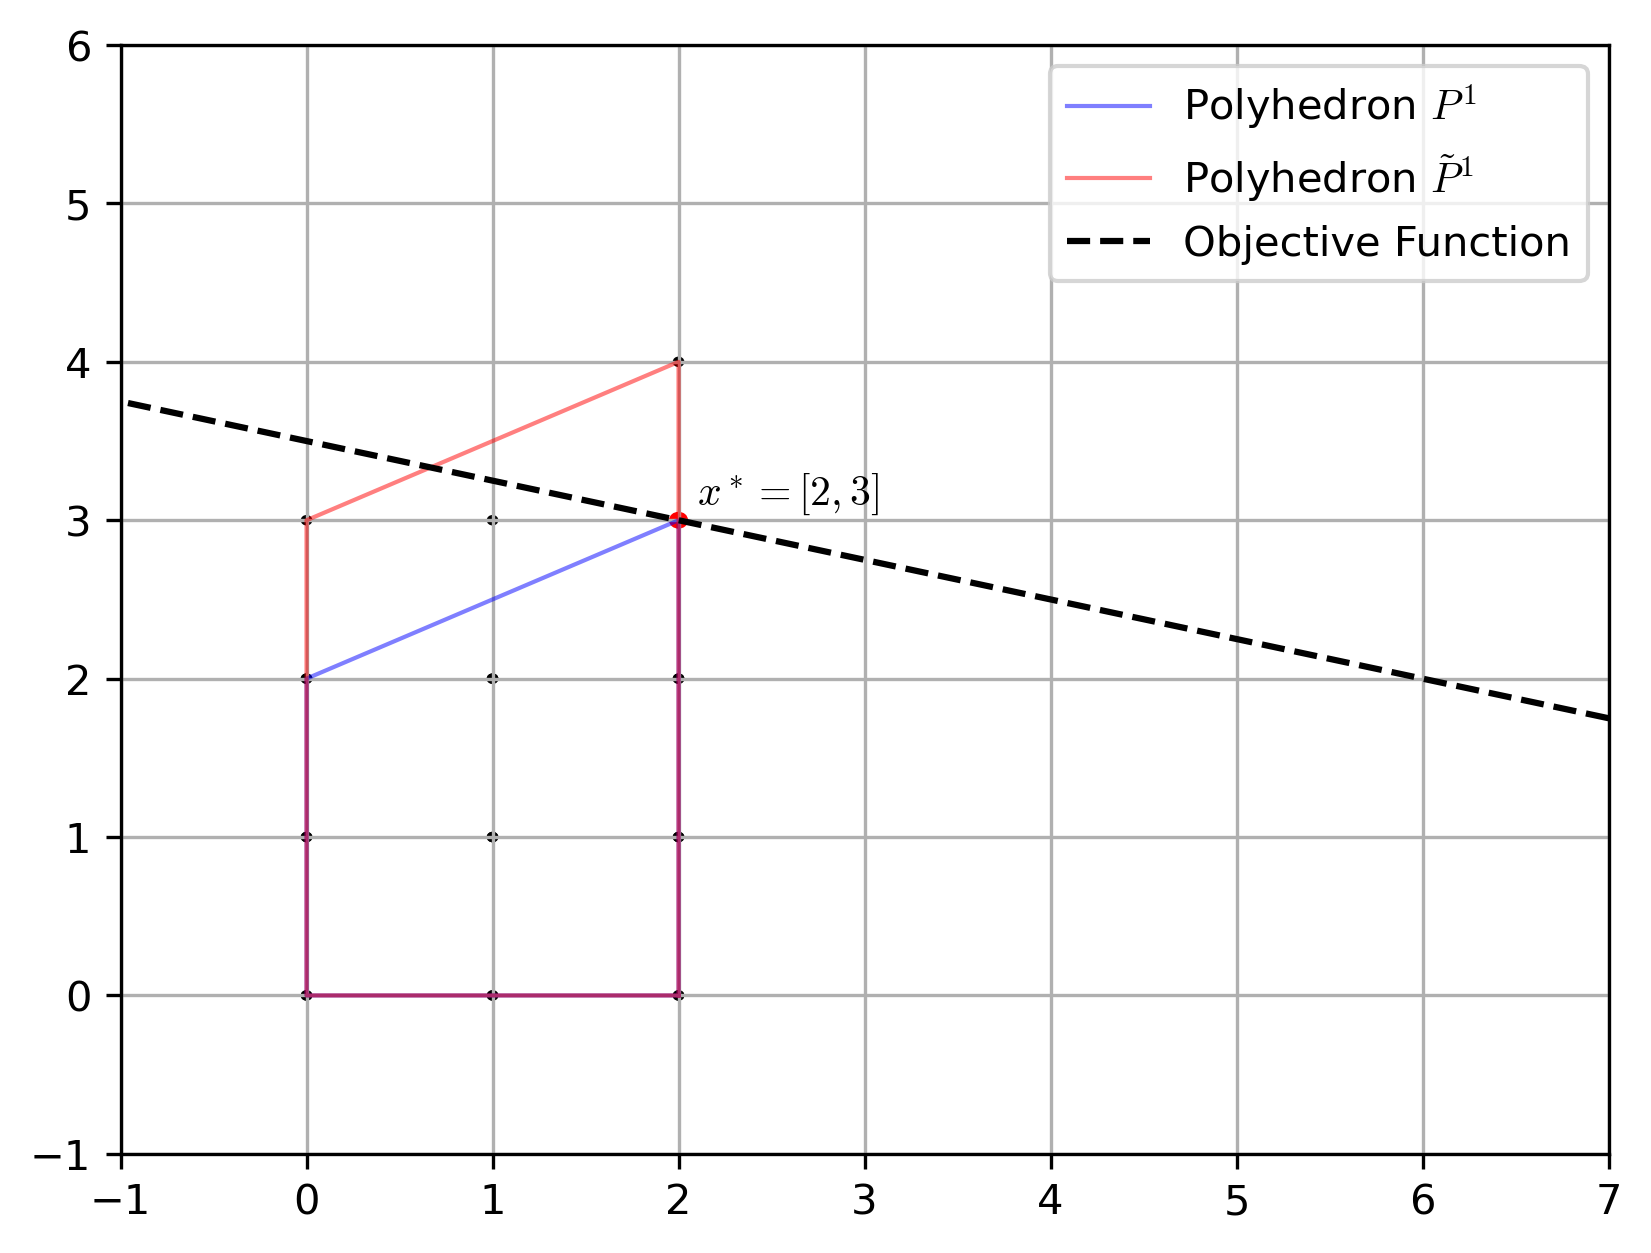
\includegraphics[width=.45\textwidth]{P1_prime.png}
					\hfill
					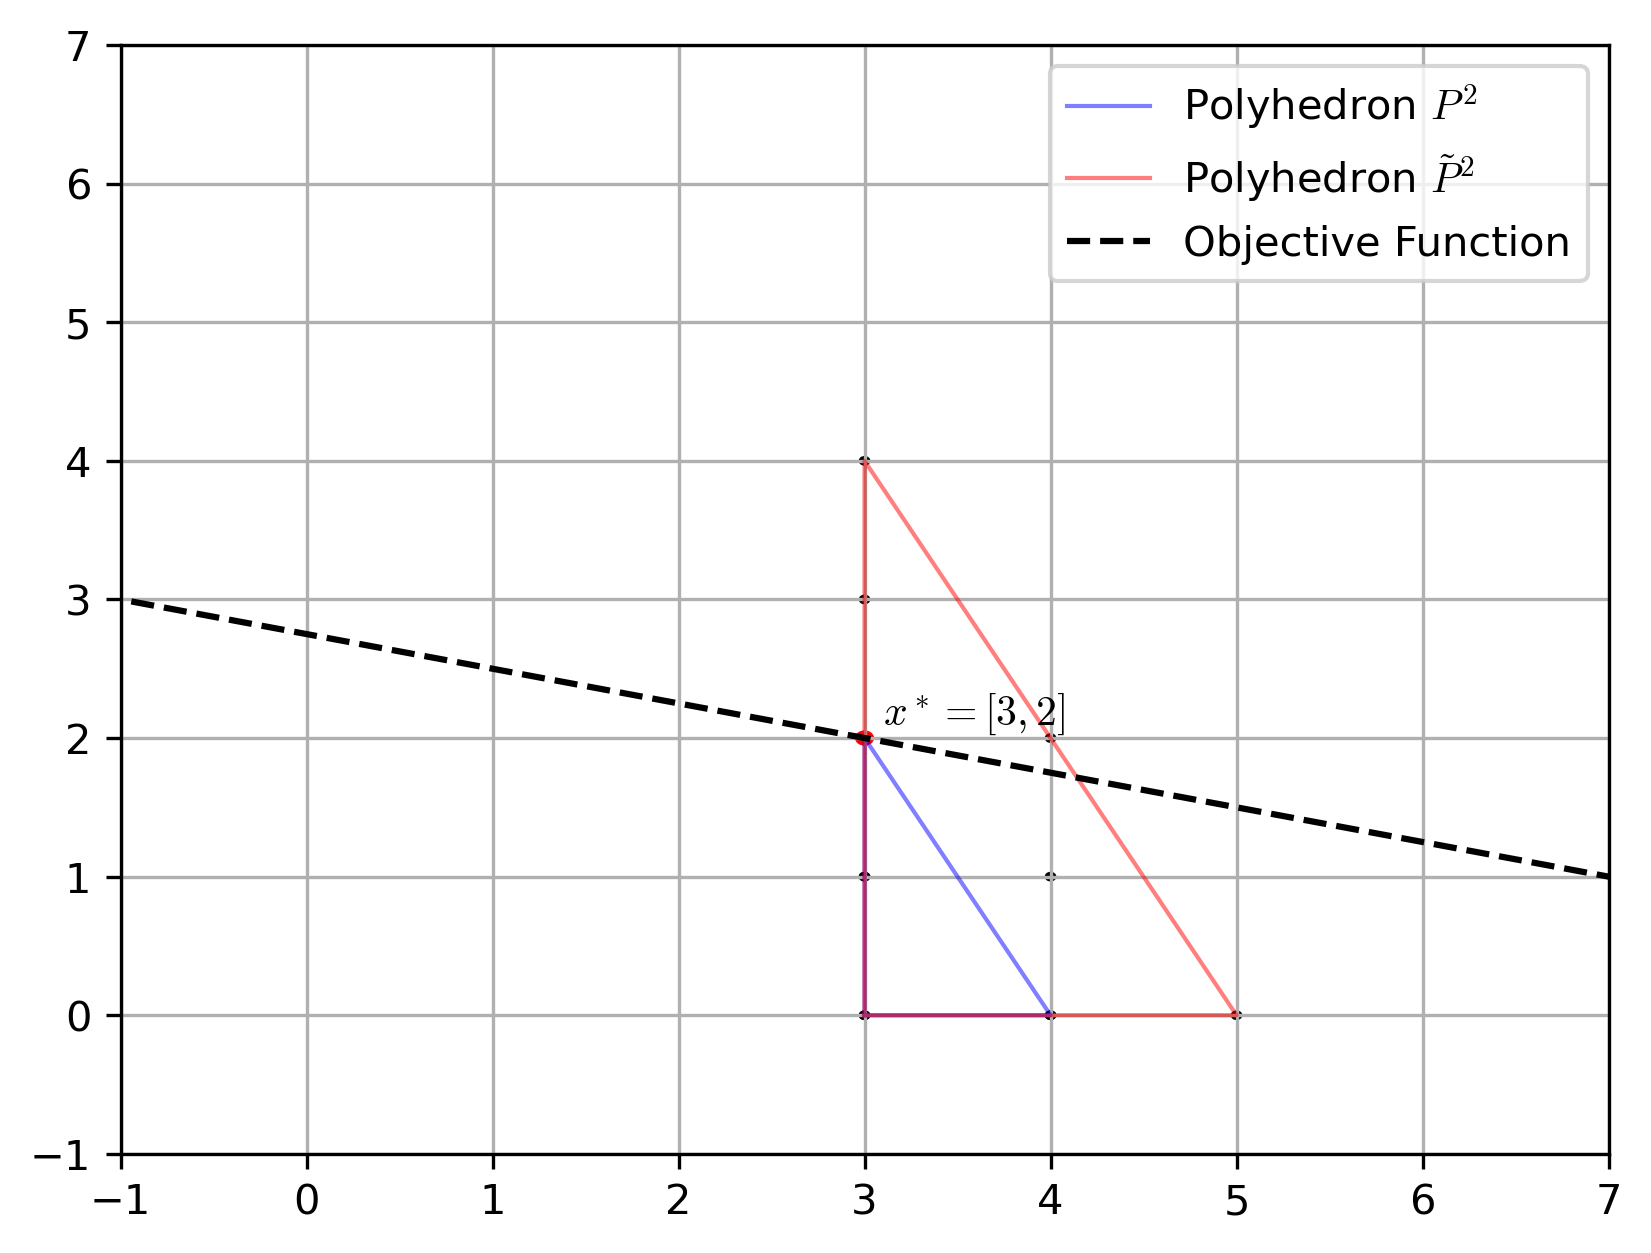
\includegraphics[width=.45\textwidth]{P2_prime.png}
					\captionsetup{font=footnotesize,labelfont=footnotesize}
					\caption{(\ref{right})'s Branch and Bound tree}
					\label{p:after}
				\end{figure}
			\end{column}
		\end{columns}
		\vspace{-.25cm}
		\begin{block}{}
			After solving (\ref{left}), we can get a tree for (\ref{right}) without another solve by substituting (\ref{right})'s bounds in each subproblem of (\ref{left}).
		\end{block}
		\normalsize
	\end{frame}

	\begin{frame}[t]
		\frametitle{A Better Warm-Starting Approach}
		\small
		\begin{columns}[T]
			% a cut valid for the subproblems of the second instance
			\begin{column}{0.4\textwidth}
				\vspace{-.25cm}
				\begin{figure}[h]
					\resizebox{\textwidth}{!}{%
						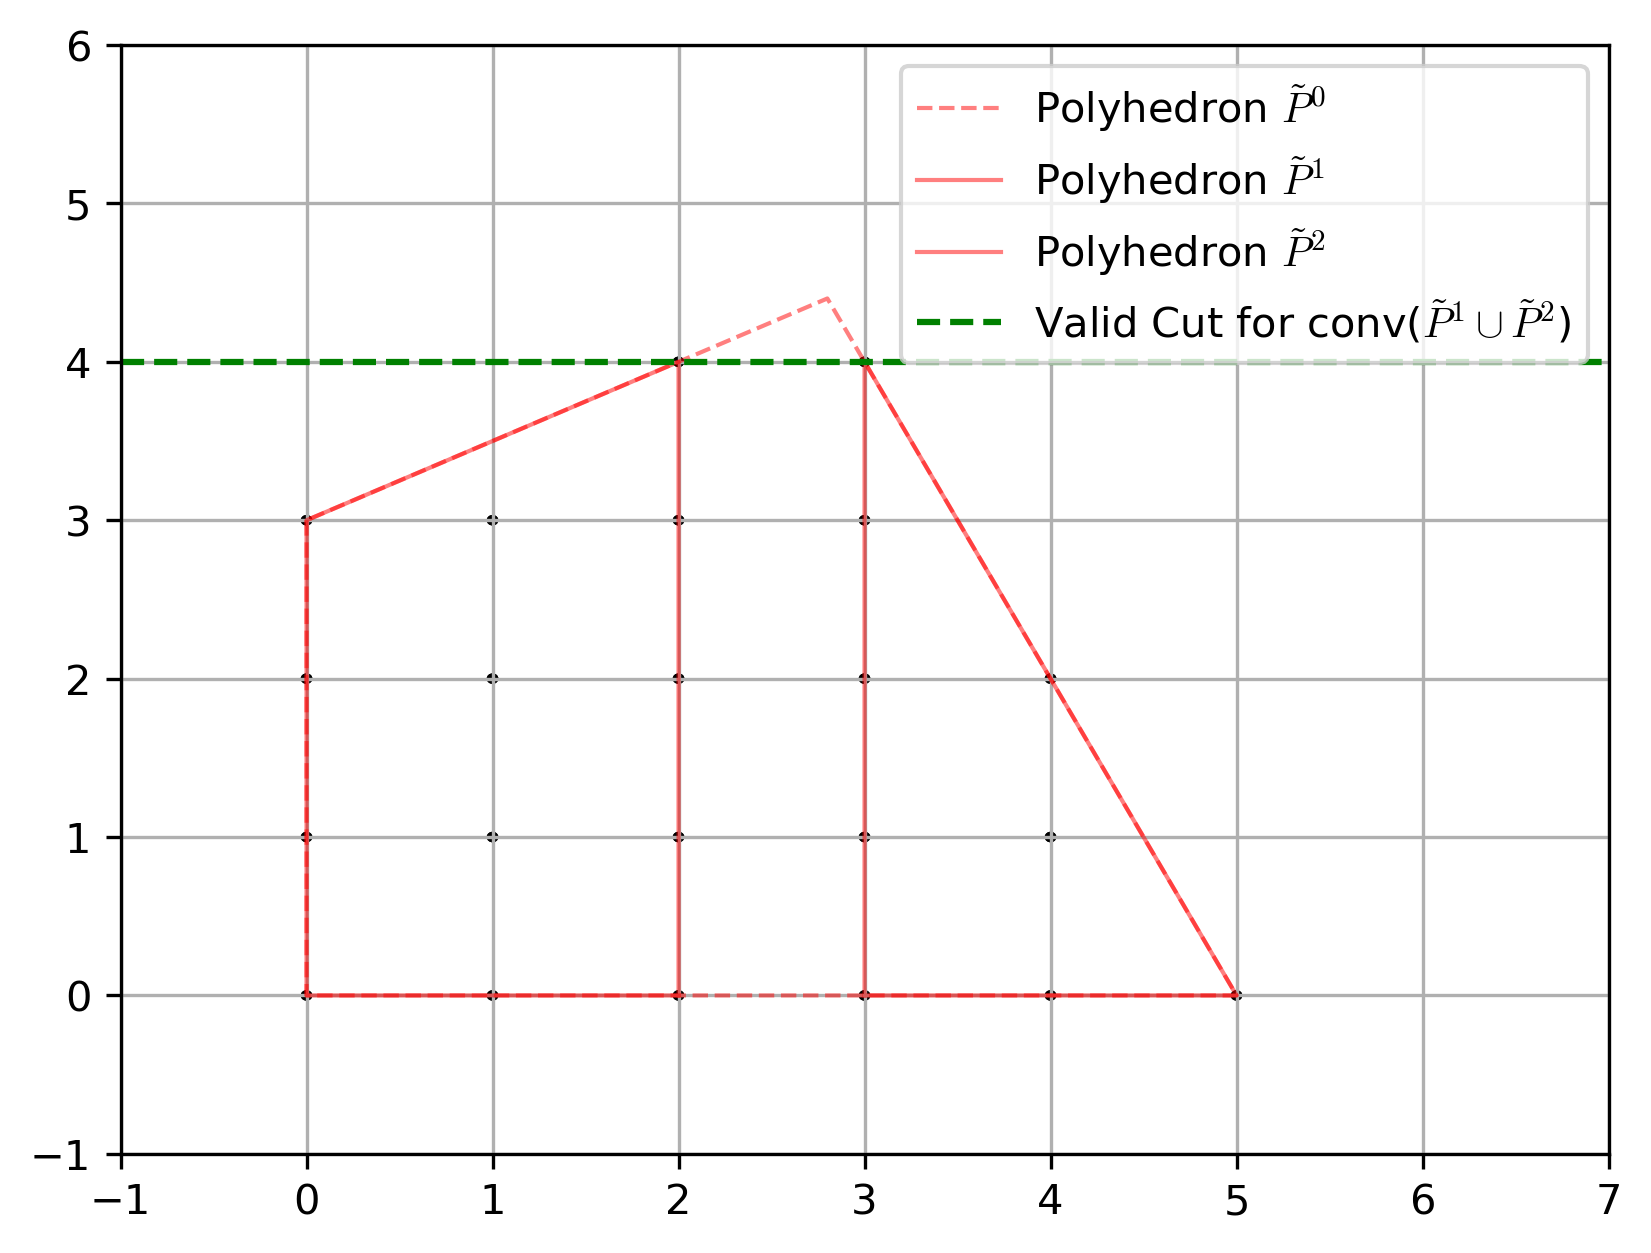
\includegraphics[]{PD_prime.png}
					}
					\caption{A cut valid for both of (\ref{right})'s subproblems}
					\label{p:hull}
				\end{figure}
			\end{column}
			\begin{column}{0.6\textwidth}
				\begin{itemize}
					\item When warm-starting, we would like to avoid:
					\begin{itemize}
						\item Reprocessing each terminal node.
						\item Refining the feasible region far from the solution.
					\end{itemize}
					\item We want to find cuts such that:
					\begin{itemize}
						\item No terminal subproblem is violated.
						\item Some estimate of the solution is maximally violated.
					\end{itemize}
					\item \cite{aleks} provides an algorithm to find such cuts.
				\end{itemize}
			\end{column}
		\end{columns}
		\vspace{.5cm}
		\begin{block}{}
			My first paper will augment this algorithm to become a cutting plane technique tightening the initial LP relaxation of MILP's in a series.
		\end{block}
		\normalsize
	\end{frame}

	\section{How to demonstrate efficiency is improved?}
	
	\begin{frame}[t]
		\frametitle{Branch and Price}
		\small
		\vspace{0cm}
		\begin{itemize}
			\item Branch and Price algorithms solve a Dantzig-Wolfe reformulation of the LP relaxation in each node.
			\item Dantzig-Wolfe relies on column generation to produce partially integer feasible solutions.
			\item The column generation subproblem is a series of MILP's.
			\item One of the most important applications is solving the Capacitated Vehicle Routing Problem with Time Windows (CVRPTW).
			\item The CVRPTW could benefit from warm-starting by:
			\begin{itemize}
				\item Outperfoming current dynamic programming subproblem formulations.
				\item Providing an efficient way to model side constraints on routes.
			\end{itemize}
		\end{itemize}
		\vspace{0cm}
		\begin{block}{}
			My second paper will demonstrate my methodology's effectiveness at improving run time and expanding modeling richness for the CVRPTW.
		\end{block}
		\normalsize
	\end{frame}

	\begin{frame}[t]
		\frametitle{Dual Decomposition for Stochastic MILP}
		\small
		\vspace{0cm}
		\begin{itemize}
			\item Dual Decomposition algorithms break stochastic MILP's into multiple independent deterministic MILP's.
			\item Each MILP is solved repeatedly with perturbed objective and constraint bounds
			\item One of the most important applications is solving the Two Stage Stochastic Unit Commitment (TSSUC).
			\item The TSSUC could benefit from warm-starting by outperfoming cold-started Lagrangian Dual formulations.
		\end{itemize}
		\vspace{1.5cm}
		\begin{block}{}
			My third paper will demonstrate my methodology's effectiveness at improving run time for the TSSUC.
		\end{block}
		\normalsize
	\end{frame}
	
	\begin{frame}[t]
		\frametitle{Conclusion}
		\small
		My dissertation will address the following research gaps:
		\begin{itemize}
			\item Overcoming current obstacles when warm-starting series of MILP's in general.
			\item The lack of warm-starting applied problems.
		\end{itemize}
		My dissertation will yield:
		\begin{itemize}
			\item A new methodology for warm-starting series of MILP's.
			\item Demonstrations of how to apply it to important real-world problems.
			\item Proof of its effectiveness in improving how such problems are solved.
		\end{itemize}
		\normalsize
	\end{frame}

	\begin{frame}[t]
		\frametitle{Status}
		\small
		\begin{columns}[T]
			% a cut valid for the subproblems of the second instance
			\begin{column}{0.5\textwidth}
				Current Items Completed:
				\begin{itemize}
					\item Theory for disjunctive cuts
					\item Plan for future research
					\item Disjunctive cuts implemented
					\item Numerical experiments implemented
				\end{itemize}
			\end{column}
			\begin{column}{0.5\textwidth}
				Items to Complete This Semester
				\begin{itemize}
					\item Clarify disjunctive cut theory
					\item Add first round of numerical experiments to paper
					\item Convert paper to poster
				\end{itemize}
			\end{column}
		\end{columns}
		\vspace{2.5cm}
		\begin{block}{}
			These deliverables will frame my remaining research work at Lehigh and enable me to quickly assemble presentation materials for conferences.
		\end{block}
		\normalsize
	\end{frame}
	
\end{document}
